\documentclass[12pt]{article}

\usepackage{graphicx}
\usepackage[margin=1.0in]{geometry}
\usepackage{amsmath}
\usepackage{cases}
\usepackage{amsfonts}
\usepackage{amssymb}
\usepackage{grffile}
\usepackage{setspace}

\setlength\parindent{0pt}

\author{Xiaohui Chen \\EID: xc2388}
\title{M 362K Post-Class Homework 6}


\begin{document}
\maketitle
\begin{spacing}{2.0}

\section*{3-1}
The probability distribution is shown below:

\begin{tabular}{|c|c|}
  \hline
  % after \\: \hline or \cline{col1-col2} \cline{col3-col4} ...
  y & $Pr(Y=y)$ \\
  \hline
  0 & $\frac{{}_{7}C_{3}}{{}_{12}C_{3}}= \frac{7}{44}$ \\
  \hline
  1 & $\frac{{}_{5}C_{1}*{}_{7}C_{2}}{{}_{12}C_{3}}= \frac{21}{44}$ \\
  \hline
  2 & $\frac{{}_{7}C_{1}*{}_{5}C_{2}}{{}_{12}C_{3}}= \frac{14}{44}$ \\
  \hline
  3 & $\frac{{}_{5}C_{3}}{{}_{12}C_{3}}= \frac{2}{44}$ \\
  \hline
\end{tabular}

\section*{3-4}

\subsection*{(a)}

The probability distribution is shown below:

\begin{tabular}{|c|c|}
  \hline
  % after \\: \hline or \cline{col1-col2} \cline{col3-col4} ...
  s & $Pr(S=s)$ \\
  \hline
  1 & $\frac{18}{38}$ \\
  \hline
  2 & $\frac{20}{38}*\frac{18}{38}$ \\
  \hline
  3 & $\left(\frac{20}{38}\right)^2*\frac{18}{38}$ \\
  \hline
  $\vdots$ & $\vdots$ \\
  \hline
  n & $\left(\frac{20}{38}\right)^{n-1}*\frac{18}{38}$ \\
  \hline
\end{tabular}

\subsection*{(b)}
We have 20 candies and 18 chewing gums. A person chooses one item at a time and put it back right after. The person stops whenever a chewing gum is selected. The probability distribution of the number of times until that person stops is the same as the situation given in this question

\section*{3-6}

\subsection*{(a)}

The probability distribution is shown below:

\begin{tabular}{|c|c|c|c|c|c|c|c|}
  \hline
  % after \\: \hline or \cline{col1-col2} \cline{col3-col4} ...
  a & 17 & 18 & 19 & 20 & 21 & 22 & 23 \\
  \hline
  $Pr(A=a)$ & 0 & 0.23 & 0.25 & 0.41 & 0.05 & 0.05 & 0.01 \\
  \hline
\end{tabular}

\subsection*{(b)}

\begin{figure}
  \centering
  % Requires \usepackage{graphicx}
  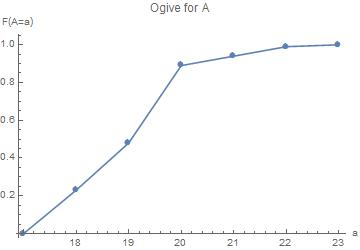
\includegraphics[width=4in]{out1}\\
  \caption{Ggive diagram for A}\label{out1}
\end{figure}

The ogive diagram is shown in Figure \ref{out1}

\section*{3-9}
Let X be the value of a house

Then $Pr(120 \le X \le 500)=0.75-0.4=0.35$

\end{spacing}
\end{document} 